\begin{figure}[htbp]
    \centering
    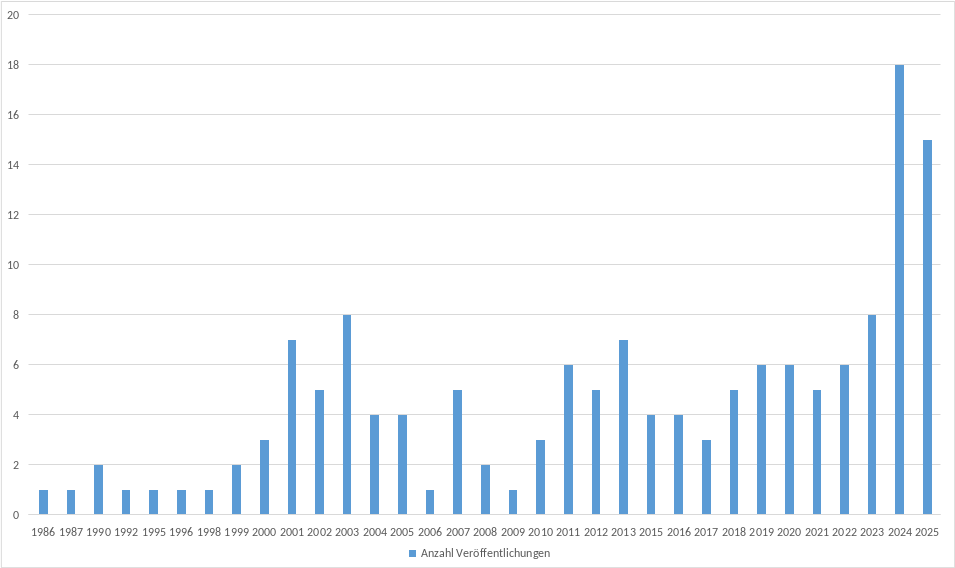
\includegraphics[width=0.90\textwidth]{graphics/1-veroeffentlichungen-jahr.png}
    \caption{Eigene Darstellung: Übersicht der Veröffentlichen pro Jahr}
    \label{fig:1-veroeffentlichungen-jahr}
\end{figure}

\begin{figure}[htbp]
    \centering
    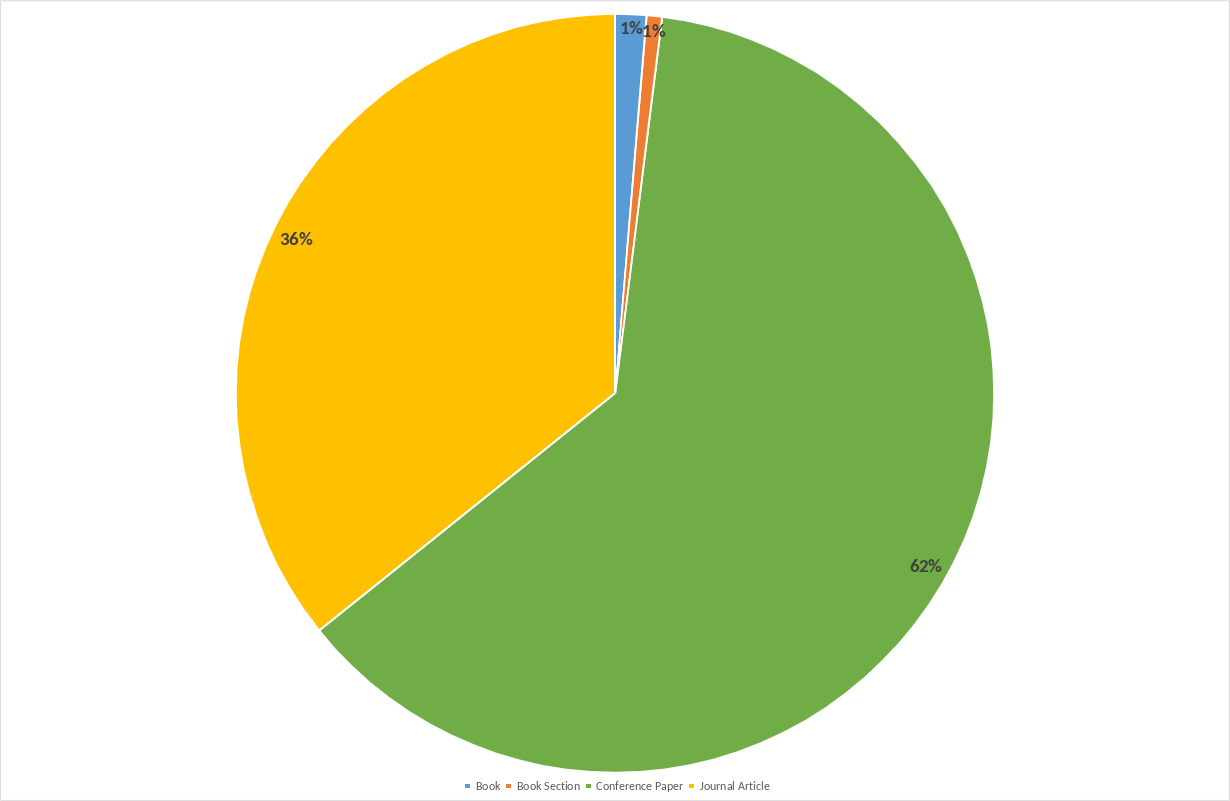
\includegraphics[width=0.90\textwidth]{graphics/2-typ.png}
    \caption{Eigene Darstellung: Übersicht des Typs aller Veröffentlichen}
    \label{fig:2-typ}
\end{figure}
